As discussed in Section~\ref{sec:runtime}, StarNet has potential to scale inference to large astronomical surveys. 
The $100\times100$ image of M2 was chosen as a test bed because a ground truth catalog
could be obtained from Hubble images for validation. 
Moreover, the our point source model is fairly realistic on M2: 
all sources are stars, and there are no galaxies in this region. 
However, most regions of the sky are much less crowded than M2.

SDSS run 94, camcol 1, field  12 is a sparse field more typical of SDSS images. 
After ten minutes of sleep training, StarNet produced a catalog on the full $1489\times 2048$ image in $\approx2$ seconds. For comparison, the projected runtime of PCAT is six days.  

This image is contained in Stripe 82, a region of the sky repeatedly imaged by SDSS. Averaging images from different runs boosts the signal to noise ratio and this {\itshape co-added} image can be analyzed to obtain a ground truth. 

However, this region of the sky also contains galaxies, which are 
not well-modelled by a PSF. A future paper will extend our generative model to include galaxies. For this experiment, only the sleep phase was employed; 
otherwise the model will try to use the PSF to explain both stars and galaxies in the wake-phase. 

Since this region of the sky is more sparse, we tile the image into $50\times 50$ tiles; $N_{max}$ on the tiles is three. 

A $500\times 500$ subimage with the StarNet catalog is shown in 
Figure~\ref{fig:sparse_field_detect}.
Figure~\ref{fig:sparse_field_tpr} reports the TPR, using the coadded catalog as ground truth. 
(We have false defections, namely galaxies, and thus 
do not report the PPV).
The StarNet TPR is comparable with the TPR of the PHOTO catalog. 
Currently, most of the missed detections occur when a large galaxy within a tile causes all $N_{max}$ detections to be placed around the galaxy -- the remaining stars in the image go undetected. 


\begin{figure}
    \centering
    \begin{subfigure}{0.45\textwidth}
        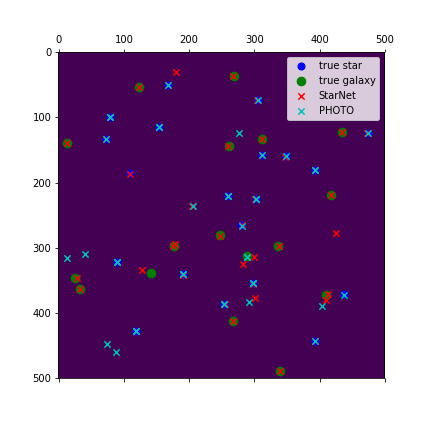
\includegraphics[width=\textwidth]{figures/sparse_field_detections.png}
        \subcaption{}
        \label{fig:sparse_field_detect}
    \end{subfigure}
    \begin{subfigure}{0.54\textwidth}
        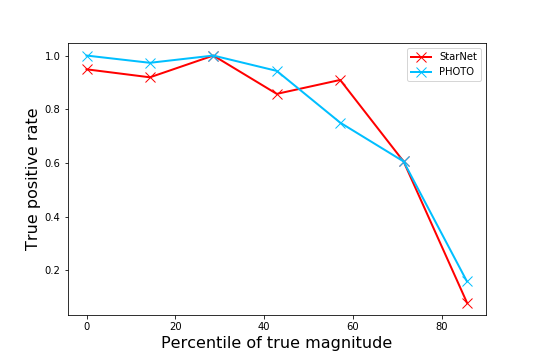
\includegraphics[width=\textwidth]{figures/sparse_field_tpr.png}
        \subcaption{}
        \label{fig:sparse_field_tpr}
    \end{subfigure}
    \caption{(a) a $500\times 500$ sparse field, with true stars in 
    blue, and true galaxies in green. Estimated stars are shown in red x's. 
    (b) the true positive rate as a function of true magnitude. }
    \label{fig:sparse_field}
\end{figure}
